\documentclass[a4paper,12pt]{article}

%%% Работа с русским языком % для pdfLatex
\usepackage{cmap}					% поиск в~PDF
\usepackage{mathtext} 				% русские буквы в~фомулах
\usepackage[T2A]{fontenc}			% кодировка
\usepackage[utf8]{inputenc}			% кодировка исходного текста
\usepackage[english,russian]{babel}	% локализация и переносы
\usepackage{indentfirst} 			% отступ 1 абзаца
\usepackage{gensymb}				% мат символы?

%%% Работа с русским языком % для XeLatex
%\usepackage[english,russian]{babel}   %% загружает пакет многоязыковой вёрстки
%\usepackage{fontspec}      %% подготавливает загрузку шрифтов Open Type, True Type и др.
%\defaultfontfeatures{Ligatures={TeX},Renderer=Basic}  %% свойства шрифтов по умолчанию
%\setmainfont[Ligatures={TeX,Historic}]{Times New Roman} %% задаёт основной шрифт документа
%\setsansfont{Comic Sans MS}                    %% задаёт шрифт без засечек
%\setmonofont{Courier New}
%\usepackage{indentfirst}
%\frenchspacing

%%% Дополнительная работа с математикой
\usepackage{amsfonts,amssymb,amsthm,mathtools}
\usepackage{amsmath}
\usepackage{icomma} % "Умная" запятая: $0,2$ --- число, $0, 2$ --- перечисление
\usepackage{upgreek}

%% Номера формул
%\mathtoolsset{showonlyrefs=true} % Показывать номера только у тех формул, на которые есть \eqref{} в~тексте.

%%% Страница
\usepackage{extsizes} % Возможность сделать 14-й шрифт

%% Шрифты
\usepackage{euscript}	 % Шрифт Евклид
\usepackage{mathrsfs} % Красивый матшрифт

%% Свои команды
\DeclareMathOperator{\sgn}{\mathop{sgn}} % создание новой конанды \sgn (типо как \sin)
\DeclareMathOperator{\rg}{\mathop{rg}}
\DeclareMathOperator{\Rg}{\mathop{Rg}}
\DeclareMathOperator{\im}{\mathop{Im}}
\DeclareMathOperator{\tr}{\mathop{tr}}
\DeclareMathOperator{\const}{\mathop{const}}
\DeclareMathOperator{\Id}{\mathop{Id}}
%\DeclareMathOperator{\dim}{\mathop{dim}}
\usepackage{csquotes} % ещё одна штука для цитат
\newcommand{\pd}[2]{\ensuremath{\cfrac{\partial #1}{\partial #2}}} % частная производная
\newcommand{\abs}[1]{\ensuremath{\left|#1\right|}} % модуль
\renewcommand{\phi}{\ensuremath{\varphi}} % греческая фи
\newcommand{\pogk}[1]{\!\left(\cfrac{\sigma_{#1}}{#1}\right)^{\!\!\!2}\!} % для погрешностей


%\renewcommand{\labelenumi}{\asbuk{enumi})}

% Ссылки
\usepackage{color} % подключить пакет color
% выбрать цвета
\definecolor{BlueGreen}{RGB}{49,152,255}
\definecolor{Violet}{RGB}{120,80,120}
% назначить цвета при подключении hyperref
\usepackage[unicode, colorlinks, urlcolor=blue, linkcolor=blue, pagecolor=blue, citecolor=blue]{hyperref} %синие ссылки
%\usepackage[unicode, colorlinks, urlcolor=black, linkcolor=black, pagecolor=black, citecolor=black]{hyperref} % для печати (отключить верхний!)


%% Перенос знаков в~формулах (по Львовскому)
\newcommand*{\hm}[1]{#1\nobreak\discretionary{}
	{\hbox{$\mathsurround=0pt #1$}}{}}

%%% Работа с картинками
\usepackage{graphicx}  % Для вставки рисунков
\graphicspath{{images/}{images2/}}  % папки с картинками
\setlength\fboxsep{3pt} % Отступ рамки \fbox{} от рисунка
\setlength\fboxrule{1pt} % Толщина линий рамки \fbox{}
\usepackage{wrapfig} % Обтекание рисунков и таблиц текстом
\usepackage{multicol}

%%% Работа с таблицами
\usepackage{array,tabularx,tabulary,booktabs} % Дополнительная работа с таблицами
\usepackage{longtable}  % Длинные таблицы
\usepackage{multirow} % Слияние строк в~таблице
\usepackage{caption}
\captionsetup{labelsep=period, labelfont=bf}

%%% Оформление
\usepackage{indentfirst} % Красная строка
%\setlength{\parskip}{0.3cm} % отступы между абзацами
%%% Название разделов
\usepackage{titlesec}
\titlelabel{\thetitle.\quad}
\renewcommand{\figurename}{\textbf{Рис.}}		%Чтобы вместо figure под рисунками писал "рис"
\renewcommand{\tablename}{\textbf{Таблица}}		%Чтобы вместо table над таблицами писал Таблица
\usepackage{enumitem}
\setlist{nolistsep}
\usepackage{verbatim}

%%% Теоремы
\theoremstyle{plain} % Это стиль по умолчанию, его можно не переопределять.
\newtheorem{theorem}{Теорема}[section]
\newtheorem{proposition}[theorem]{Утверждение}
\newtheorem{predlog}{Предложение}[section]
\newtheorem{lemma}{Лемма}[section]

\theoremstyle{definition} % "Определение"
\newtheorem{definition}{Определение}[section]
\newtheorem{corollary}{Следствие}[theorem]
\newtheorem{problem}{Задача}[section]

\theoremstyle{remark} % "Примечание"
\newtheorem*{nonum}{Решение}
\newtheorem{zamech}{Замечание}[theorem]

%%% Правильные мат. символы для русского языка
\renewcommand{\epsilon}{\ensuremath{\varepsilon}}
\renewcommand{\phi}{\ensuremath{\varphi}}
\renewcommand{\kappa}{\ensuremath{\varkappa}}
\renewcommand{\le}{\ensuremath{\leqslant}}
\renewcommand{\leq}{\ensuremath{\leqslant}}
\renewcommand{\ge}{\ensuremath{\geqslant}}
\renewcommand{\geq}{\ensuremath{\geqslant}}
\renewcommand{\emptyset}{\varnothing}

%%% Для лекций по инфе
\usepackage{alltt}
\newcounter{infa}[section]
\newcounter{num}
\definecolor{infa}{rgb}{0, 0.2, 0.89}
\definecolor{infa1}{rgb}{0, 0.3, 1}
\definecolor{grey}{rgb}{0.5, 0.5, 0.5}
\newcommand{\tab}{\ \ \ }
\newcommand{\com}[1]{{\color{grey}\##1}}
\newcommand{\num}{\addtocounter{num}{1}\arabic{num}\tab}
\newcommand{\defi}{{\color{infa}def}}
\newcommand{\ini}{{\color{infa}in}}
\newcommand{\rangei}{{\color{infa}range}}
\newcommand{\fori}{{\color{infa}for}}
\newcommand{\ifi}{{\color{infa}if}}
\newcommand{\elsei}{{\color{infa}else}}
\newcommand{\printi}{{\color{infa1}print}}
\newcommand{\maxi}{{\color{infa}max}}
\newcommand{\classi}{{\color{infa}class}}
\newcommand{\returni}{{\color{infa}return}}
\newcommand{\elifi}{{\color{infa}elif}}


\newenvironment{infa}[1]{
	
	\vspace{0.5cm}
	\addtocounter{infa}{1}%
	\noindent{\large \textbf{Программа №\thesection.\arabic{infa}}}\textbf{<<#1>>}%
	\begin{alltt}%
	}{\end{alltt}
	\setcounter{num}{0}
	\vspace{0.1cm}}
%Пример кода:
%\begin{infa}{Поразрядная сортировка}
%	\ \num \defi count_sort(a):\tab \com{определяет нашу функцию}
%	\ \num \tab m = \maxi(a)+1
%	\ \num \tab q = [0]*m
%	\ \num \tab \fori x \ini a:
%	\ \num \tab \tab q[x] += 1
%	\ \num \tab pos = 0
%	\ \num \tab \fori x \ini q:
%	\ \num \tab \tab \fori i \ini \rangei(q[x]):
%	\ \num \tab \tab \tab a[pos] = x
%	\num \tab \tab \tab pos += 1
%\end{infa}

\usepackage{titlesec}
\titlelabel{\thetitle.\quad}


\usepackage{graphicx,xcolor,adjustbox,setspace}

\newcommand{\resh}{\noindent\textit{Решение:}\\}

\newcounter{prim}
\newenvironment{prim}{%
	\addtocounter{prim}{1}
	\noindent{\\
		\textbf{\noindentПример \arabic{prim}\\}}%
}{\vspace{2mm}\\
	\resh
}
\definecolor{orange}{rgb}{1, 0.7, 0.1}
%\usepackage{ulem}

\usepackage{bm} %жирный греческий шрифт

\newenvironment{psm}
{\left(\begin{smallmatrix*}[r]}
	{\end{smallmatrix*}\right)}

\newenvironment{pmatrixr}
{\begin{pmatrix*}[r]}
	{\end{pmatrix*}}

\renewcommand{\figurename}{\textbf{Рис.}}		%Чтобы вместо figure под рисунками писал "рис"
\renewcommand{\tablename}{\textbf{Таблица}}		%Чтобы вместо table над таблицами писал Таблица


\title{3.4.2}
\author{Кутушева Алиса}
\date{today}
\usepackage[left=1.27cm,right=1.27cm,top=1.27cm,bottom=2cm]{geometry}
\begin{document}
	
	\begin{titlepage}
		\begin{center} 
			
			\large Московский физико-технический институт\\
			Факультет молекулярной и химической физики\\
			\vspace{7cm}
			\huge Лабораторная работа № 3.4.2\\
			\textbf{\Large <<Закон Кюри-Вейсса>>}\\
		\end{center} 
		
		\vspace{7.5cm}
		{\par \raggedleft \large \emph{Выполнили:}\\ студенты 2 курса\\ 641 группы ФМХФ\\ Кутушева Алиса\\ Ильдаровна \\ \& \\Горшков Тимофей \\Владимирович \par}
		\begin{center}
			\vfill Москва 2017
		\end{center}
	\end{titlepage}
\newpage
\setcounter{page}{2}

\begin{center}
	\vspace*{-0.5cm}{
		\textbf{Аннотация:}\\ 
		\vspace{0.2cm}
		\parbox{16cm}{ 
			\tab В~этом отчёте изложены результаты выполнения лабораторной работы <<Закон Кюри-Вейсса>>. В данной работе изучается температурная зависимость $\chi$(T) магнитной проницаемости гадолиния при температурах выше точки Кюри. Путем исследования зависимости периода колебаний автогенератора от температуры сердечника катушки определяется парамагнитная точка Кюри гадолиния.
		}
	}
\end{center}

	\hspace{0.2cm}\textbf{Цель работы:}
	\par изучение температурной зависимости магнитной восприимчивости ферромагнетика выше точки Кюри.


	\hspace{0.2cm}\textbf{В работе используются:}
	\par катушка самоиндукции с образцом из гальдония, термостат, частотометр, цифровой вольтметр, LC-автогенератор, термопара медь-константан.
	
\par \textbf{Теоретические сведения:}
\par Вещества с отличными от нуля атомными магнитными моментами обладают парамагнитными свойствами. Внешнее магнитное поле ориентирует магнитные моменты, которые в отсутствие поля располагались в пространстве хаотичным образом.
\par При повышении температуры Т возрастает дезориентируещее действие теплового движения частиц, и магнитная восприимчивость парамагнетиков убывает, в простейшем случае (в постоянном магнитном поле) — по закону Кюри:
\begin{equation}
\chi = C/T,
\end{equation} где С — постоянная Кюри.

\begin{wrapfigure}{r}{0.4\textwidth}
	\centering
	\fbox{
		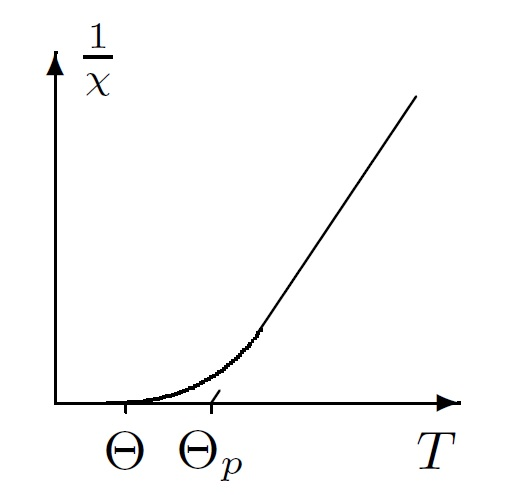
\includegraphics[width=\linewidth]{K_V1}}
	\caption{Зависимость обратной величины магнитной восприимчивости от температуры}
	\label{mah}
\end{wrapfigure}

\par Для парамагнитных веществ, которые при понижении температуры становятся ферромагнитными, формула (1) должна быть видоизменена. Эта формула показывает, что температура Т = 0 является особой точкой температурной кривой, в которой х неограниченно возрастает.
При Т $\to$ 0 тепловое движение всё меньше препятствует магнитным моментам атомов ориентироваться в одном направлении при сколь угодно слабом внешнем поле. В ферромагнетиках — под влиянием обменных сил — это происходит при понижении температуры не до абсолютного нуля, а до температуры Кюри $\Theta$. Оказывается, что у ферромагнетиков закон Кюри должен быть заменён законом Кюри—Вейсса:
\begin{equation}
\chi \sim \frac{1}{T-\Theta_p},
\end{equation}
\par где $\Theta_p$ — температура, близкая к температуре
Кюри.
Эта формула хорошо описывает поведение ферромагнитных веществ после их перехода в парамагнитную фазу при заметном удалении температуры от 0, но недостаточно точна при Т $\approx \Theta_p$.
Иногда для уточнения формулы (2) вводят вместо одной две температуры Кюри, одна из которых описывает точку фазового перехода — ферромагнитная точка Кюри $\Theta$, а другая является параметром в формуле (2) — парамагнитная точка Кюри — $\Theta_p$ (рис. 1).

\par \textbf{Экспериментальная установка:}
\begin{figure}
	\centering
	\fbox{
		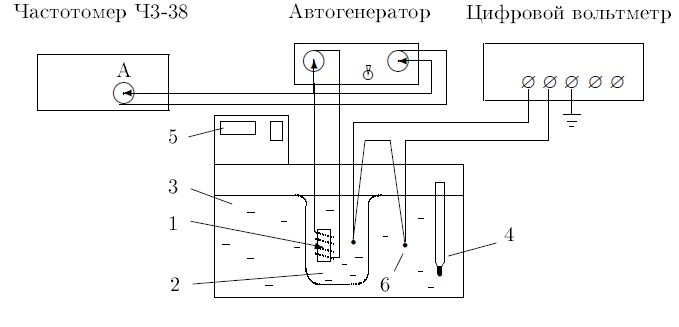
\includegraphics[width=\linewidth]{K_V2}}
	\caption{Схема экспериментальной установки}
	\label{mah}

\end{figure}
\par Схема установки для проверки закона Кюри-Вейсса показана на рис.2. Исследуемый ферромагнитный образец (гадолиний) расположен внутри пустотелой катушки самоиндукции, которая служит индуктивностью колебательного контура, входящего в состав LC-автогенератора. Автогенератор собран на полевом транзисторе КП-103 и смонтирован в виде отдельного блока.
\par Гадолиний является хорошим проводником электрического тока, а рабочая частота генератора достаточно велика (~50 кГц), поэтому для уменьшения вихревых токов образец изготовлен из мелких кусочков размером около 0,5 мм. Катушка 1 с образцом помещена в стеклянный сосуд 2, залитый трансформаторным маслом. Масло предохраняет образец от окисления и способствует ухудшению электрического контакта между отдельными частичками образца. Кроме того, оно улучшает тепловой контакт между образцом и термостатируемой (рабочей) жидкостью 3 в термостате. Ртутный термометр 4 используется для приближённой оценки температуры. Температура образца регулируется с помощью термостата.
Рассчитаем температуру Т образца с учётом показаний термопары и величину $1/(\tau^2 - \tau_0^2)$, данные занесем в таблицу 1. Построим график зависимости $1/(\tau^{2} - \tau_0^2) = f(T)$. Экстраполируя полученную прямую к оси абсцисс, определим парамагнитную точку Кюри $\Theta_p$ для гадолиния.
\par Магнитная восприимчивость образца х определяется по изменению самоиндукции катушки. Обозначив через L самоиндукцию катушки с образцом и через $L_0$ — её самоиндукцию в отсутствие образца, получим:
\begin{equation}
(L-L_0) \sim \chi
\end{equation}
При изменении самоиндукции образца меняется период колебаний автогенератора:
\begin{equation}
\tau = 2 \pi \sqrt {LC}
\end{equation}
где С — ёмкость контура автогенератора.
Период колебаний в отсутствие образца определяется самоиндукцией пустой катушки:
\begin{equation}
\tau = 2 \pi \sqrt {L_0C}
\end{equation}
Из (4) и (5) имеем
\begin{equation}
(L-L_0) \sim (\tau^2 - \tau_0^2)
\end{equation}
Таким образом,
\begin{equation}
\chi \sim (\tau^2 - \tau_0^2)
\end{equation}
Из формул (2) и (7) следует, что закон Кюри-Вейсса справедлив, если выполнено соотношение:
\begin{equation}
\frac {1}{\chi} \sim (T-\Theta_p) \sim \frac{1}{(\tau^2 - \tau_0^2)}
\end{equation}
\par \textbf{Ход работы:}
\par 1. Подготовим приборы к работе.
\par 2. Оценим допустимую ЭДС термопары (допустимая разность температур образца и рабочей жидкости $\Delta T = 0.5$ \degree C, постоянная термопары k = 24 град/мВ):
\begin{equation}
	\varepsilon = \frac{\Delta T}{k} = \frac {0.5}{24} = 0.021 \text{ мВ}
\end{equation}
\par 3. Исследуем зависимость периода колебаний LС-генератора от температуры образца, отмечая период колебаний $\tau$ по частотомеру, а температуру Т — по показаниям дисплея и цифровому вольтметру ($\Delta$U с учётом знака). Термопара подключена так, что при знаке «+» на табло вольтметра температура образца выше температуры рабочей жидкости.
Проведем измерения в диапазоне от 14 \degree С до 40 \degree С через 2 \degree С. Занесем данные в таблицу 1.
Запишем период колебаний $\tau_0$ без образца, указанный на установке: $\tau_0$ = 9.050 мкс.
\begin{table}[h!]
	\centering
	\caption{ Экспериментальные данные }

\begin{tabular}{|c|c|c|c|c|c|}
	\hline 
	\rule[0ex]{0pt}{2.5ex} № & $T_0$, К & $\tau$, мкс & $\Delta U$, мВ & T, K & $\frac{1}{\tau^2-\tau_0 ^2}, 10^{12} c^{-2}$ \\
	\hline 
	1 & 288 & 10.780 & 0.001 & 288.024 & 0.02915 \\
	\hline 
	2 & 290 & 10.681 & -0.021 & 289.496 & 0.03107 \\ 
	\hline 
	3 & 292 & 10.494 & -0.021 & 291.496 & 0.03543 \\ 
	\hline 
	4 & 294 & 10.213 & -0.016 & 293.616 & 0.04464 \\ 
	\hline 
	5 & 296 & 9.877 & -0.018 & 295.568 & 0.06389 \\
	\hline 
	6 & 298 & 9.563 & -0.019 & 297.544 & 0.10473 \\
	\hline 
	7 & 300 & 9.392 & -0.012 & 299.712 & 0.15855 \\
	\hline 
	8 & 302 & 9.324 & -0.015 & 301.64 & 0.19863 \\
	\hline 
	9 & 304 & 9.279 & -0.015 & 303.64 & 0.23825 \\
	\hline 
	10 & 306 & 9.247 & -0.021 & 305.496 & 0.27743 \\ 
	\hline 
	11 & 308 & 9.221 & -0.017 & 307.592 & 0.32007 \\
	\hline 
	12 & 310 & 9.201 & -0.015 & 309.64 & 0.36286 \\
	\hline 
	13 & 312 & 9.187 & -0.015 & 311.64 & 0.40025 \\
	\hline 
\end{tabular} 
\end{table}
	\\
	\hspace{0.2cm}\textbf{Обратка результатов:}

\par 1. Рассчитаем температуру Т образца с учётом показаний термопары и величину $ \frac {1}{(\tau^2 - \tau_0^2)}$, данные занесем в таблицу 1. Построим график зависимости $ \frac {1}{(\tau^2 - \tau_0^2)} = f(T)$. 
\begin{figure}
	\centering
	\fbox{
		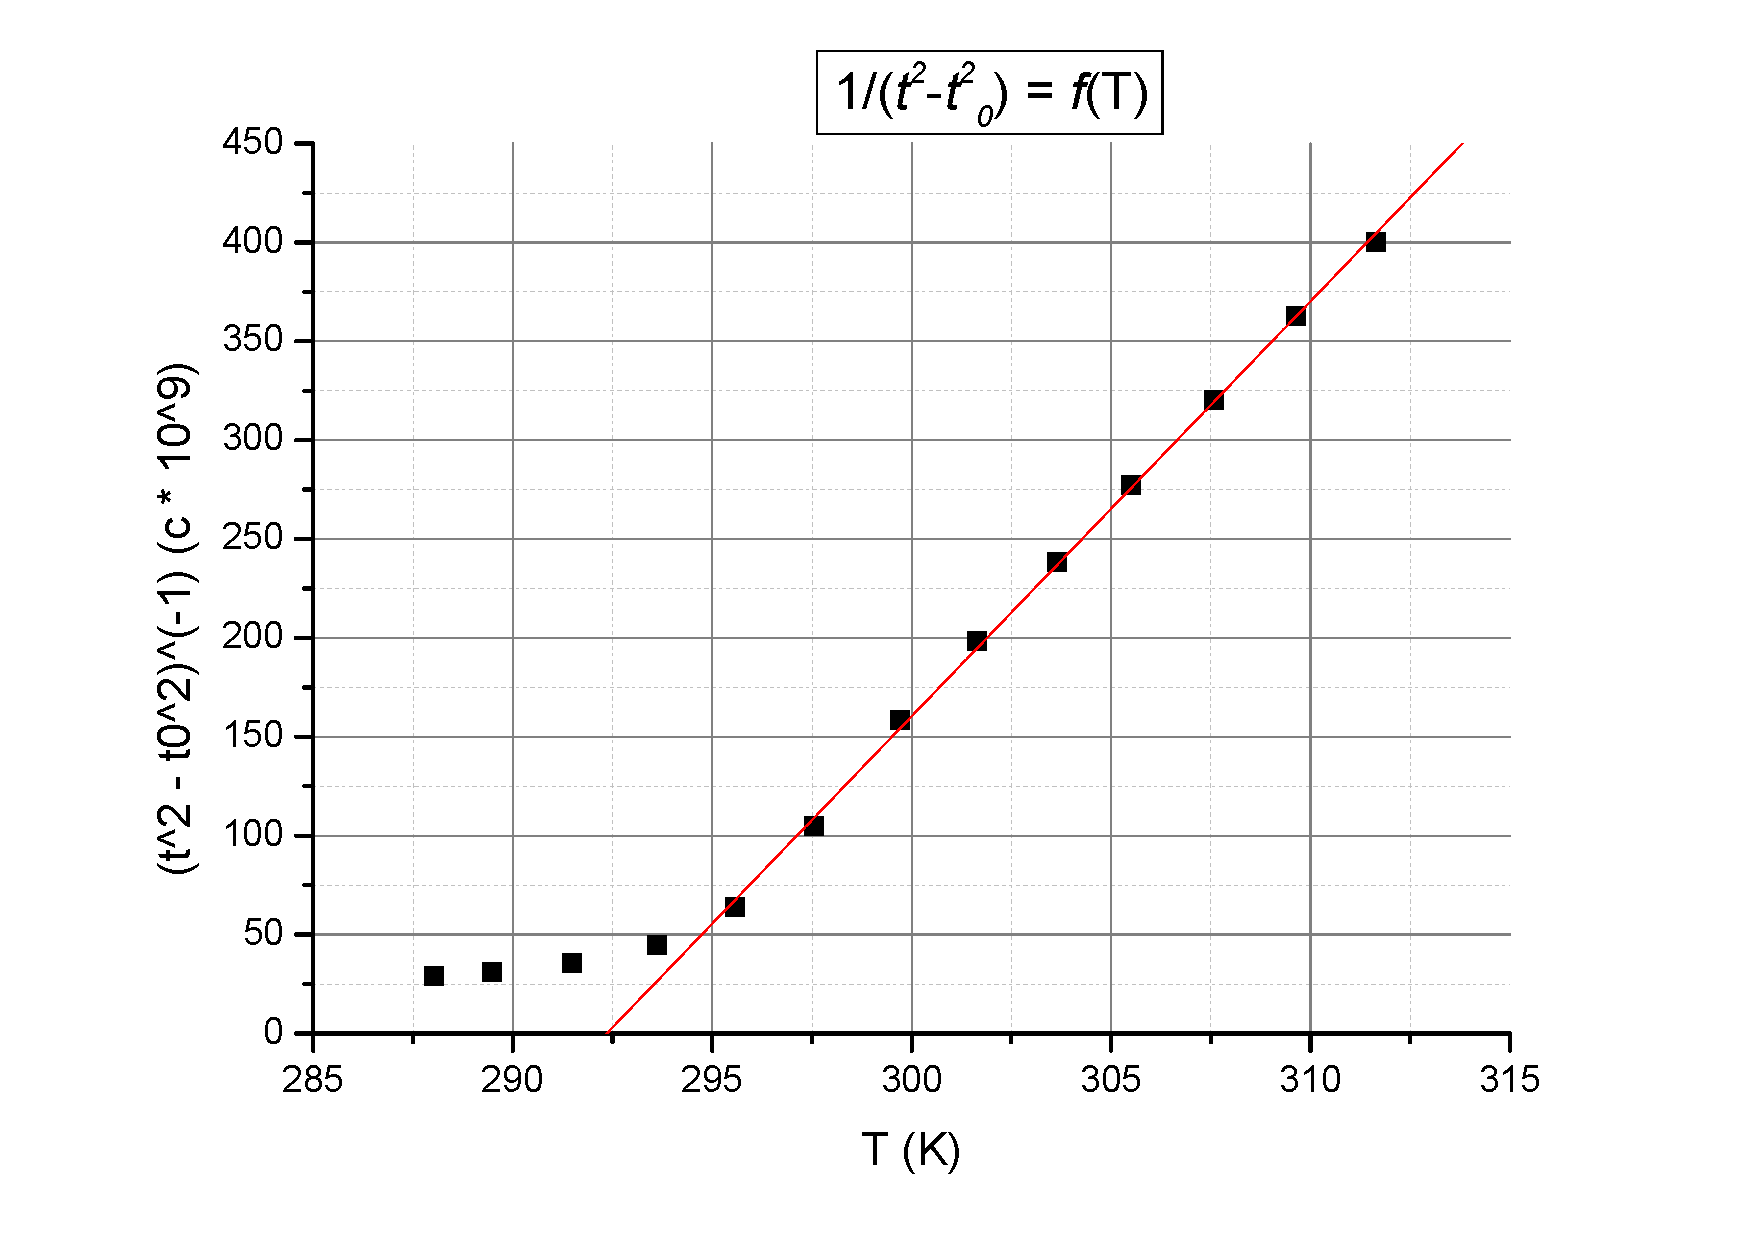
\includegraphics[width=\linewidth]{K_V3}}
	\caption{ График экстраполируемой зависимости}
	\label{mah}
\end{figure}
Экстраполируя полученную прямую к оси абсцисс, определим парамагнитную точку Кюри $\Theta_p$ для гадолиния.

f(T) = k*T + b, где $k = (21.0 \pm 0.2)*10^9$, а $b = (-6130 \pm 70)*10^9$.
$\Theta_p = - \left (\frac{b}{k} \right) = \frac {6130}{21} = 291.9 K$
\par 2. Оценим погрешности эксперимента и сравним результат с табличным. Для частного погрешность рассчитывается по формуле (10):
\begin{equation}
{\varepsilon_\Theta}_p = \sqrt{\left({\varepsilon_a}^2+{\varepsilon_b}^2\right)} 
\end{equation}
\begin{equation}
	dT = \Theta_p*\sqrt{\left(\left(\frac{db}{b}\right)^2+\left(\frac{dk}{k}\right)^2\right)}  = 291.9*\sqrt{\left(\left(\frac{70}{6130}\right)^2+\left(\frac{0.2}{21}\right)^2\right)} = 4
\end{equation}
\par $\Theta_p = 292 \pm 4 K$.
\par Табличное значение: $\Theta_p = 289 K$.
\par \textbf{Вывод:}
\par В ходе данной работы исходя из теоретических пропорциональностей было экстраполировано значение парамагнитной точки Кюри. Табличное значение $\Theta_p = 289 K$ попало в доверительный интервал истинных значений: $\Theta_p = 292 \pm 4 K$. Значение относительной погрешности составило ${\varepsilon_\Theta}_p = \frac {dT}{\Theta_p} * 100\% = \frac {4}{292} * 100\% = 1.4\%$
\end{document}